Современные интеллектуальные ассистенты являются многокомпонентными системами, организующими
среду взаимодействия, целевой сценарий диалога, персонализацию и приватность переписки. Конкретные компоненты
выбираются исходя из целей и возможностей команды разработчиков. Для исследовательских целей, как правило, используется
открытое программное обеспечение, требующее лишь незначительной адаптации под постановку. В этой секции 
будет описан подход к созданию цифрового ассистента для проведения исследования. 

Основой современных ассистентов является большая языковая модель, обученная посредством техник оптимизации выполнять
инструкции, описанные естественным языком. Модель прекрасно справляется с задачами коммуникации, придерживается делового
этикета и демонстрирует эмпатическое внимание к проблемам пользователя \cite{jiang2023mistral}\cite{llamatouvron2023}.

Языковая модель также помогает в решении повседневных и деловых задач, выделяя наиболее важное из академических статей и помогая составлять
планы проектов. Последние достижения позволяют задавать вопросы по изображениям, что существенно облегчает выбор продуктов, например одежды или мебели
\cite{bai2023qwen}. Тем не менее современные ассистенты не способны к выполнению формальных логических операций: 
арифметических действий \cite{bubeck2023sparks}, решению абстрактных логических задач \cite{bordt2023chatgpt}, соблюдению правил стратегических игр \cite{Adam2024}.

\begin{figure}[h]
    \centering
    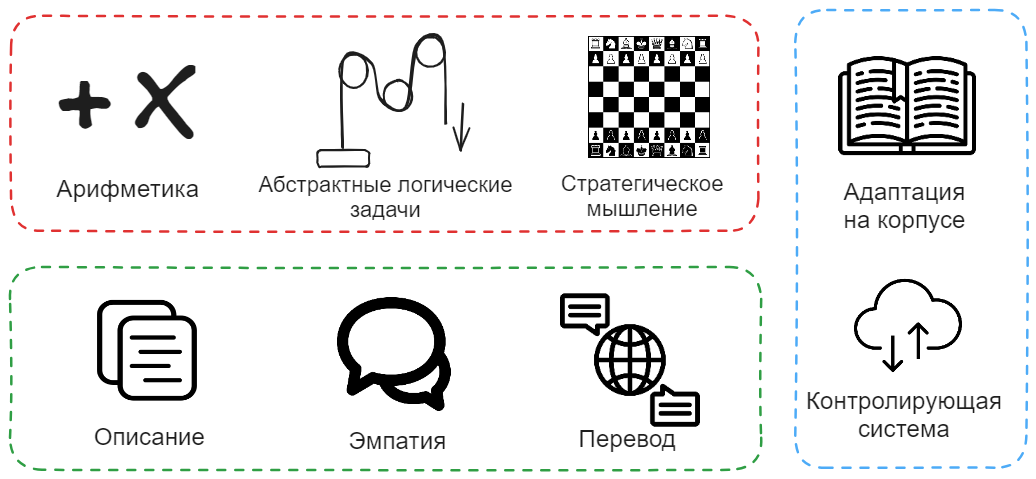
\includegraphics[width=0.7\textwidth]{assets/work/arch/problems.excalidraw.png}
    \caption{Навыки современного ассистента ограничены коммуникацией и решением базовых задач обработки текста}
    \label{problems}
\end{figure}

В образовании интеллектуальные ассистенты применяются для обучения языку \cite{аль2019интеллектуальный} и рисования поясняющих графиков \cite{bulusuautomated}. 
Примерами коммерческого использования ассистентов в образовании являются компании Merlin Mind и OpenAI Education. Ключевым преимуществом решений 
является адаптация к государственным общеобразовательным программам, взаимодействие с интерактивной доской и проприетарно подготовленная база знаний, 
регулярно обновляемая предметными экспертами.
